\chapter{Origins}
\label{ch:origins}

\section{Proto-economics}
\textbf{Trigger warning: Many of the quotes in this section are rather racist.} \\

Economics conventionally starts with the publication of Adam Smith's \emph{The Wealth of Nations} in 1776. Before that, however, many anticipated what later became elements of economics.

In those early days, agriculture was the dominant sector in the economy. Production was production of food, trade was trade in food, consumption was consumption of food. These proto-economists, like all farmers, were keenly aware of the importance of climate and geography. Cato (c160 BCE), Varro (37 BCE), Columella (41-68) and Palladius (c400) all wrote handbooks on farm management. 

In those days, teleology was common: Things were as they should be. Cicero \href{https://penelope.uchicago.edu/Thayer/E/Roman/Texts/Cicero/de_Officiis/1E*.html}{(44 BCE, On Duties, I 42 151)} argues that
\begin{quote}
    of all the occupations by which gain is secured, none is better than agriculture, none more profitable, none more delightful, none more becoming to a free man
\end{quote}
Cicero was writing about large landowners, not about farmhands or peasants. He argued that the landowning elite, which dominated Rome politically and economically, was morally superior. Those on top deserved to be on top.

\subsection{Environmental determinism}
Ancient scholars did not just think that the natural environment was important. They thought it was predominant. For instance, Hippocrates \href{http://classics.mit.edu/Hippocrates/airwatpl.23.23.html}{(400 BCE, On Airs, Waters, Places, 23)} wrote
\begin{quote}
The other races in Europe differ from one another, both as to stature and shape, owing to the changes of the seasons, which are very great and frequent, and because the heat is strong, the winters severe, and there are frequent rains, and again protracted droughts, and winds, from which many and diversified changes are induced. These changes are likely to have an effect upon generation in the coagulation of the semen, as this process cannot be the same in summer as in winter, nor in rainy as in dry weather; wherefore, I think, that the figures of Europeans differ more than those of Asiatics; and they differ very much from one another as to stature in the same city; for vitiations of the semen occur in its coagulation more frequently during frequent changes of the seasons, than where they are alike and equable. And the same may be said of their dispositions, for the wild, and unsociable, and the passionate occur in such a constitution; for frequent excitement of the mind induces wildness, and extinguishes sociableness and mildness of disposition, and therefore I think the inhabitants of Europe more courageous than those of Asia; for a climate which is always the same induces indolence, but a changeable climate, laborious exertions both of body and mind; and from rest and indolence cowardice is engendered, and from laborious exertions and pains, courage. On this account the inhabitants of Europe are than the Asiatics, and also owing to their institutions, because they are not governed by kings like the latter, for where men are governed by kings there they must be very cowardly, as I have stated before; for their souls are enslaved, and they will not willingly, or readily undergo dangers in order to promote the power of another; but those that are free undertake dangers on their own account, and not for the sake of others; they court hazard and go out to meet it, for they themselves bear off the rewards of victory, and thus their institutions contribute not a little to their courage.
\end{quote}
Hippocrates' prediction that Europeans can never have absolute monarchs is wrong in retrospect. Note that he argues that there are all sorts of things wrong with non-Greek Europeans and Asiatics\textemdash because of where they live\textemdash implying that the climate in Greece is responsible for the superiority of him and his countrymen.

Aristotle \href{http://classics.mit.edu/Aristotle/politics.7.seven.html}{(350 BCE, Politics, 7 VII)} wrote
\begin{quote}
    Those who live in a cold climate and in Europe are full of spirit, but wanting in intelligence and skill; and therefore they retain comparative freedom, but have no political organization, and are incapable of ruling over others. Whereas the natives of Asia are intelligent and inventive, but they are wanting in spirit, and therefore they are always in a state of subjection and slavery. But the Hellenic race, which is situated between them, is likewise intermediate in character, being high-spirited and also intelligent. Hence it continues free, and is the best-governed of any nation, and, if it could be formed into one state, would be able to rule the world.
\end{quote}
Aristotle predicted that Europeans could never rule over others. While he foresaw the empire of Alexander the Great, he missed the empires founded by Romans, Franks, Spaniards, Portuguese, Dutch, English, French, and Russians. Like Hippocrates, he argued that his own people were superior by virtue of their climate.

The ancient Greeks were not alone. In an important, early Chinese text, Zhong Guan \href{https://books.google.co.uk/books?id=Yu7eDwAAQBAJ\&pg=PA106&lpg=PA106&dq=guanzi+greedy,+uncouth,+and+warlike\&source=bl\&ots=6eLMGGPbXp\&sig=ACfU3U1ckHgtbfjTESsSPRnWIziRpLRvIQ\&hl=en\&sa=X\&ved=2ahUKEwiDqpqljZrqAhUSZcAKHWNkCCIQ6AEwAHoECAkQAQ#v=onepage\&q=guanzi\%20greedy\%2C\%20uncouth\%2C\%20and\%20warlike\&f=false}{(780 BCE, Guanzi, XIV 39)} writes
\begin{quote}
    What is water? It is the root of all things and the ancestral hall of all life. It is that from which beauty and ugliness, worthiness and unworthiness, stupidity and giftedness are produced.
    
    How do we know this to be so? Now the water of Qi is forceful, swift and twisting. Therefore its people are greedy, uncouth and warlike. The water of Chu is gentle, yielding, and pure. Therefore its people are lighthearted, resolute, and sure of themselves. The water of Yue is turbid, sluggish, and soaks the land. Therefore its people are stupid, disease ridden, and filthy. The water of Qin is thick like gruel and stagnant. It is obstructed, choked with silt, and wanders in confusion free of its banks. Therefore its people are greedy, violent, and deceptive, and they like to meddle in affairs. The water of Jin is bitter, harsh, and polluted. Therefore its people are flattering and deceitful, cunning and profit seeking. The water of Yan collects in low places and is weak. It sinks into the ground, is clogged, and wanders in confusion free of its banks. Therefore its people are stupid, idiotic, and given to divination. They treat disease lightly and die readily. The water of Song is light, strong, and pure. Therefore its people are simple and at ease with themselves, and they like things to be done in the correct way. For this reason, the sages' transformation in the world lay in understanding water.
    
    Now, when the water is unadulterated, people's hearts will be correct, they have no desire to be corrupt. When people's hearts are at easy, their conduct will never be depraved. For this reason, the sages' bringing good order to the world did not lie in preaching to every person or persuading every household, but in taking water as their central concern.
\end{quote}
The idea that you are what river shore you dwell on, seems odd to us. But note that Zhong Guan argues that you should not appeal to people's innate goodness. Instead, a wise ruler improves water courses. He so justifies the elite in a hydraulic society, whose main role was to provide public goods in water management.

The idea of environmental determinism lingered. Ibn Khaldun \href{http://www.muslimphilosophy.com/ik/Muqaddimah/Chapter1/Ch_1_04.htm}{(1377, Muqaddimah 1 4)}
\begin{quote}
We have seen that Negroes are in general characterized by levity, excitability, and great emotionalism. They are found eager to dance whenever they hear a melody. They are everywhere described as stupid. The real reason for these (opinions) is that, as has been shown by philosophers in the proper place, joy and gladness are due to expansion and diffusion of the animal spirit. Sadness is due to the opposite, namely, contraction and concentration of the animal spirit. It has been shown that heat expands and rarefies air and vapors and increases their quantity. [...]

Now, Negroes live in the hot zone (of the earth). Heat dominates their
temperament and formation. Therefore, they have in their spirits an amount of heat corresponding to that in their bodies and that of the zone in which they live. In comparison with the spirits of the inhabitants of the fourth zone,\footnote{Ibn Khaldun split the world into seven climate zones. The fourth zone, the middle one, had the optimal climate. Other zones were too hot or too cold. Ibn Khaldun lived in the optimal climate.} theirs are hotter and, consequently, more expanded. As a result, they are more quickly moved to joy and gladness, and they are merrier. Excitability is the direct consequence.

In the same way, the inhabitants of coastal regions are somewhat similar to the inhabitants of the south. The air in which they live is very much hotter because of the reflection of the light and the rays of (the sun from) the surface of the sea. Therefore, their share in the qualities resulting from heat, that is, joy and levity, is larger than that of the (inhabitants of) cold and hilly or mountainous countries. To a degree, this may be observed in the inhabitants of the Jarid in the third zone. The heat is abundant in it and in the air there, since it lies south of the coastal plains and hills. Another example is furnished by the Egyptians. Egypt lies at about the same latitude as the Jarid. The Egyptians are dominated by joyfulness, levity, and disregard for the future. They store no provisions of food, neither for a month nor a year ahead, but purchase most of it (daily) in the market. Fez in the Maghrib, on the other hand, lies inland (and is) surrounded by cold hills. Its inhabitants can be observed to look sad and gloomy and to be too much concerned for the future. Although a man in Fez might have provisions of wheat stored, sufficient to last him for years, he always goes to the market early to buy his food for the day, because he is afraid to consume any of his hoarded food.

If one pays attention to this sort of thing in the various zones and countries, the influence of the varying quality of the air upon the character (of the inhabitants) will become apparent. God is the Creator, the Knowing One. Al-Masudi undertook to investigate the reason for the levity, excitability, and emotionalism in Negroes, and attempted to explain it. However, he did no better than to report, on the authority of Galen and Ya'qub b. Ishaq al Kind!, that the reason is a weakness of their brains which results in a weakness of their intellect. This is an inconclusive and unproven statement. God guides whomever He wants to guide.
\end{quote}
Like Hippocrates and Aristotle, Ibn Khaldun argued that his climate was the best. He adds Cicero's teleology. Arabs were superior because Allah had bestowed them with the optimal climate. The dominant position of Arabs was not by happenstance, but God's will.

Ibn Khaldun's sentiment is reflected in the expression \emph{God's own country}, which has been used to describe, amongst others, Kerala, Yorkshire, and Rhodesia. Robert Rankin mockingly places the Garden of Eden in Brentford.

Montesquieu \href{https://oll.libertyfund.org/titles/montesquieu-complete-works-vol-1-the-spirit-of-laws}{(1748, The Spirit of Laws, 1 XIV)} argues that the climate of France is best. He writes that
\begin{quote}
    [...] the temper of the mind and the passions of the heart are extremely different in different climates [...]
    
    People are therefore more vigorous in cold climates. [...] In cold countries they have very little sensibility for pleasure; in temperate countries they have more; in warm countries their sensibility is exquisite. [...]
    
    In northern climates, scarcely has the animal part of love a power of making itself felt. In temperate climates, love, attended by a thousand appendages, endeavours to please by things that have, at first, the appearance, though not the reality, of this passion. In warmer climates, it is liked for its own sake, it is the only cause of happiness, it is life itself.
\end{quote}
In other words, only the French have the right mix of strength and purpose.

More than 200 years later, Huntington \href{https://www.questia.com/read/9043355/civilization-and-climate}{(1915, Civilization and Climate)} wrote
\begin{quote}
    Today a certain peculiar type of climate prevails wherever civilization is high. IN the past, the same type seems to have prevailed wherever a great civilization arose.
\end{quote}
Huntington's main innovation on earlier environmental determinists was that he argued that climate is not static. Instead, climate changes. Huntington argued that climate changes people:
\begin{quote}
    In tropical countries weakness of will is unfortunately a quality displayed not only by the natives, but by a large proportion of the northerner sojourners. If manifests itself in many ways. Four of these, namely, lack of industry, an irascible temper, drunkenness, and sexual indulgence are particularly prominent, and may be taken as typical.
\end{quote}
At the same time, he argued that
\begin{quote}
    the effect of a diverse inheritance would last indefinitely
\end{quote}
in a thought experiment about "Teutons" and "negroes" moving to an empty country much like Egypt.

It was only in 1922 that Lucien Febvre started the intellectual push back against environmental determinism. It is now an uncommon position in the social sciences. Indeed, the racist and self-serving reasoning of the early environmental determinists render it disreputable in the eyes of many of our contemporaries.

That said, environmental determinism has not disappeared. Jared Diamond (a physiologist by training) is probably the most prominent of current environmental determinists.

\subsection{Early concerns about pollution}
Early scholars wrote about the natural environment and its effect on society. Environmental pollution and resource degradation recognized too. Ancient Greece and Turkey, for instance, suffered from deforestation and soil erosion. Of his native Atticam Plato \href{http://classics.mit.edu/Plato/critias.html}{(Critias, 360 BCE)} wrote
\begin{quote}
    its mountains were high hills covered with soil, and the plains [...] were full of rich earth, and there was abundance of wood in the mountains.
\end{quote}
but
\begin{quote}
   now losing the water which flows off the bare earth into the sea 
\end{quote}
That is, Plato understood the relationship between deforestation, soil erosion, and water run-off. Visitors to modern Greece may wonder how such a barren landscape could have supported such a rich civilisation. It did not. Greece was not barren then.

Rome and its empire suffered from lead poisoning in water and air, but they themselves were not aware of this. Air pollution was more easily detected. Seneca (61) wrote about
\begin{quote}
    the heavy air of Rome, from the stink of the chimneys and the pestilence, vapors and soot of the air.
\end{quote} 

Environmental policy also goes way back. As the price of fuel wood rose in London, people switched to sea coal, bituminous coal mined on the northeast coast of England. King Edward I of England banned sea coal in 1307. Nonetheless, smog continued to plague London. In December 1952, some 4,000 people were killed by air pollution and maybe 8,000 more in the following months. The Clean Air Act of 1956 marks the beginning of the transition away from coal as the prime fuel for heating in the cities of the UK.

Marquis de Condorcet (1776), remembered in economics for his work on voting, wrote of stubble burning that
\begin{quote}
    by corrupting the air, causes illnesses in neighboring homes.
\end{quote}
This may be the first formulation of an externality, the unintended and uncompensated impact of an economic activity on a third party. Stubble burning is still a big problem, regularly causing major air pollution on the Indian subcontinent.

\section{Classical economics}

\subsection{Adam Smith on public goods}
Adam Smith's 1776 book \emph{An Inquiry into the Nature and Causes of the Wealth of Nations} is often seen as the starting point of economics as a separate discipline.

Smith is seen as a proponent of laissez-faire, the idea that the government should not intervene much in the economy, particularly through the doctrine of the invisible hand, in which the market coordinates selfish interests to deliver the social good.\footnote{You have one chance to make a first impression. Lay people typically think that Smith's views on economic policy are shared by all economists. This is peculiar, because Karl Marx was an eminent economist too. After World War II, many economists advocated central planning.} We now call this the First Fundamental Welfare Theorem. We recognize that it only holds under rather stringent conditions, and that Smith's social good is a Pareto optimum.

Smith \href{https://en.wikisource.org/wiki/The_Wealth_of_Nations/Book_V/Chapter_1#Part_3:_Of_the_Expense_of_Public_Works_and_Public_Institutions}{(Wealth of Nations, 1776 V 1)} did argue, though, that
\begin{quote}
    The third and last duty of the sovereign or commonwealth is that of erecting and maintaining those public institutions and those public works, which, though they may be in the highest degree advantageous to a great society, are, however, of such a nature that the profit could never repay the expense to any individual or small number of individuals, and which it therefore cannot be expected that any individual or small number of individuals should erect or maintain. [...] The performance of this duty requires, too, very different degrees of expense in the different periods of society.
    
    After the public institutions and public works necessary for the defence of the society, and for the administration of justice, both of which have already been mentioned, the other works and institutions of this kind are chiefly those for facilitating the commerce of the society [such as good roads, bridges, navigable canals, harbours], and those for promoting the instruction of the people.
\end{quote}
Smith realized that the market underprovides public goods, and called for government intervention.

\subsection{Malthus, Ricardo and Mill on resource limits}
\label{sc:malthus}
Thomas Robert Malthus \href{http://www.esp.org/books/malthus/population/malthus.pdf}{(1798, An Essay on the Principle of Population)} wrote
\begin{quote}
    Population, when unchecked, increases in a geometrical ratio. Subsistence increases only in an arithmetical ratio.
\end{quote}
Figure \ref{fig:malthus} illustrates this. The supply of food increases linearly or arithmetically. The number of people, and so the demand for food increases exponentially or geometrically. Exponential growth is faster than linear growth. We will therefore run out of food at some point in the future, the \emph{Malthusian Catastrophe}.\footnote{Thomas Carlyle \href{https://books.google.co.uk/books?id=UNbMBgAAQBAJ}{(1839, Chartism)} referred to Malthus' work as "[d]reary, stolid, dismal, without hope for this world or the next". Carlyle \href{https://books.google.co.uk/books?id=UNbMBgAAQBAJ}{(1849, The Negro Question)} coined the term \emph{the dismal science} in 1849, dismal in "find[ing] the secret of this Universe in 'supply and demand', and reducing the duty of human governors to that of letting men alone". Carlyle argued for slavery. Carlyle's suggestion was resisted by, among others, John Stuart Mill.}

Malthus had a solution too: Abstinence. At that time, you could not have babies without sex.

\begin{figure}
    \centering
    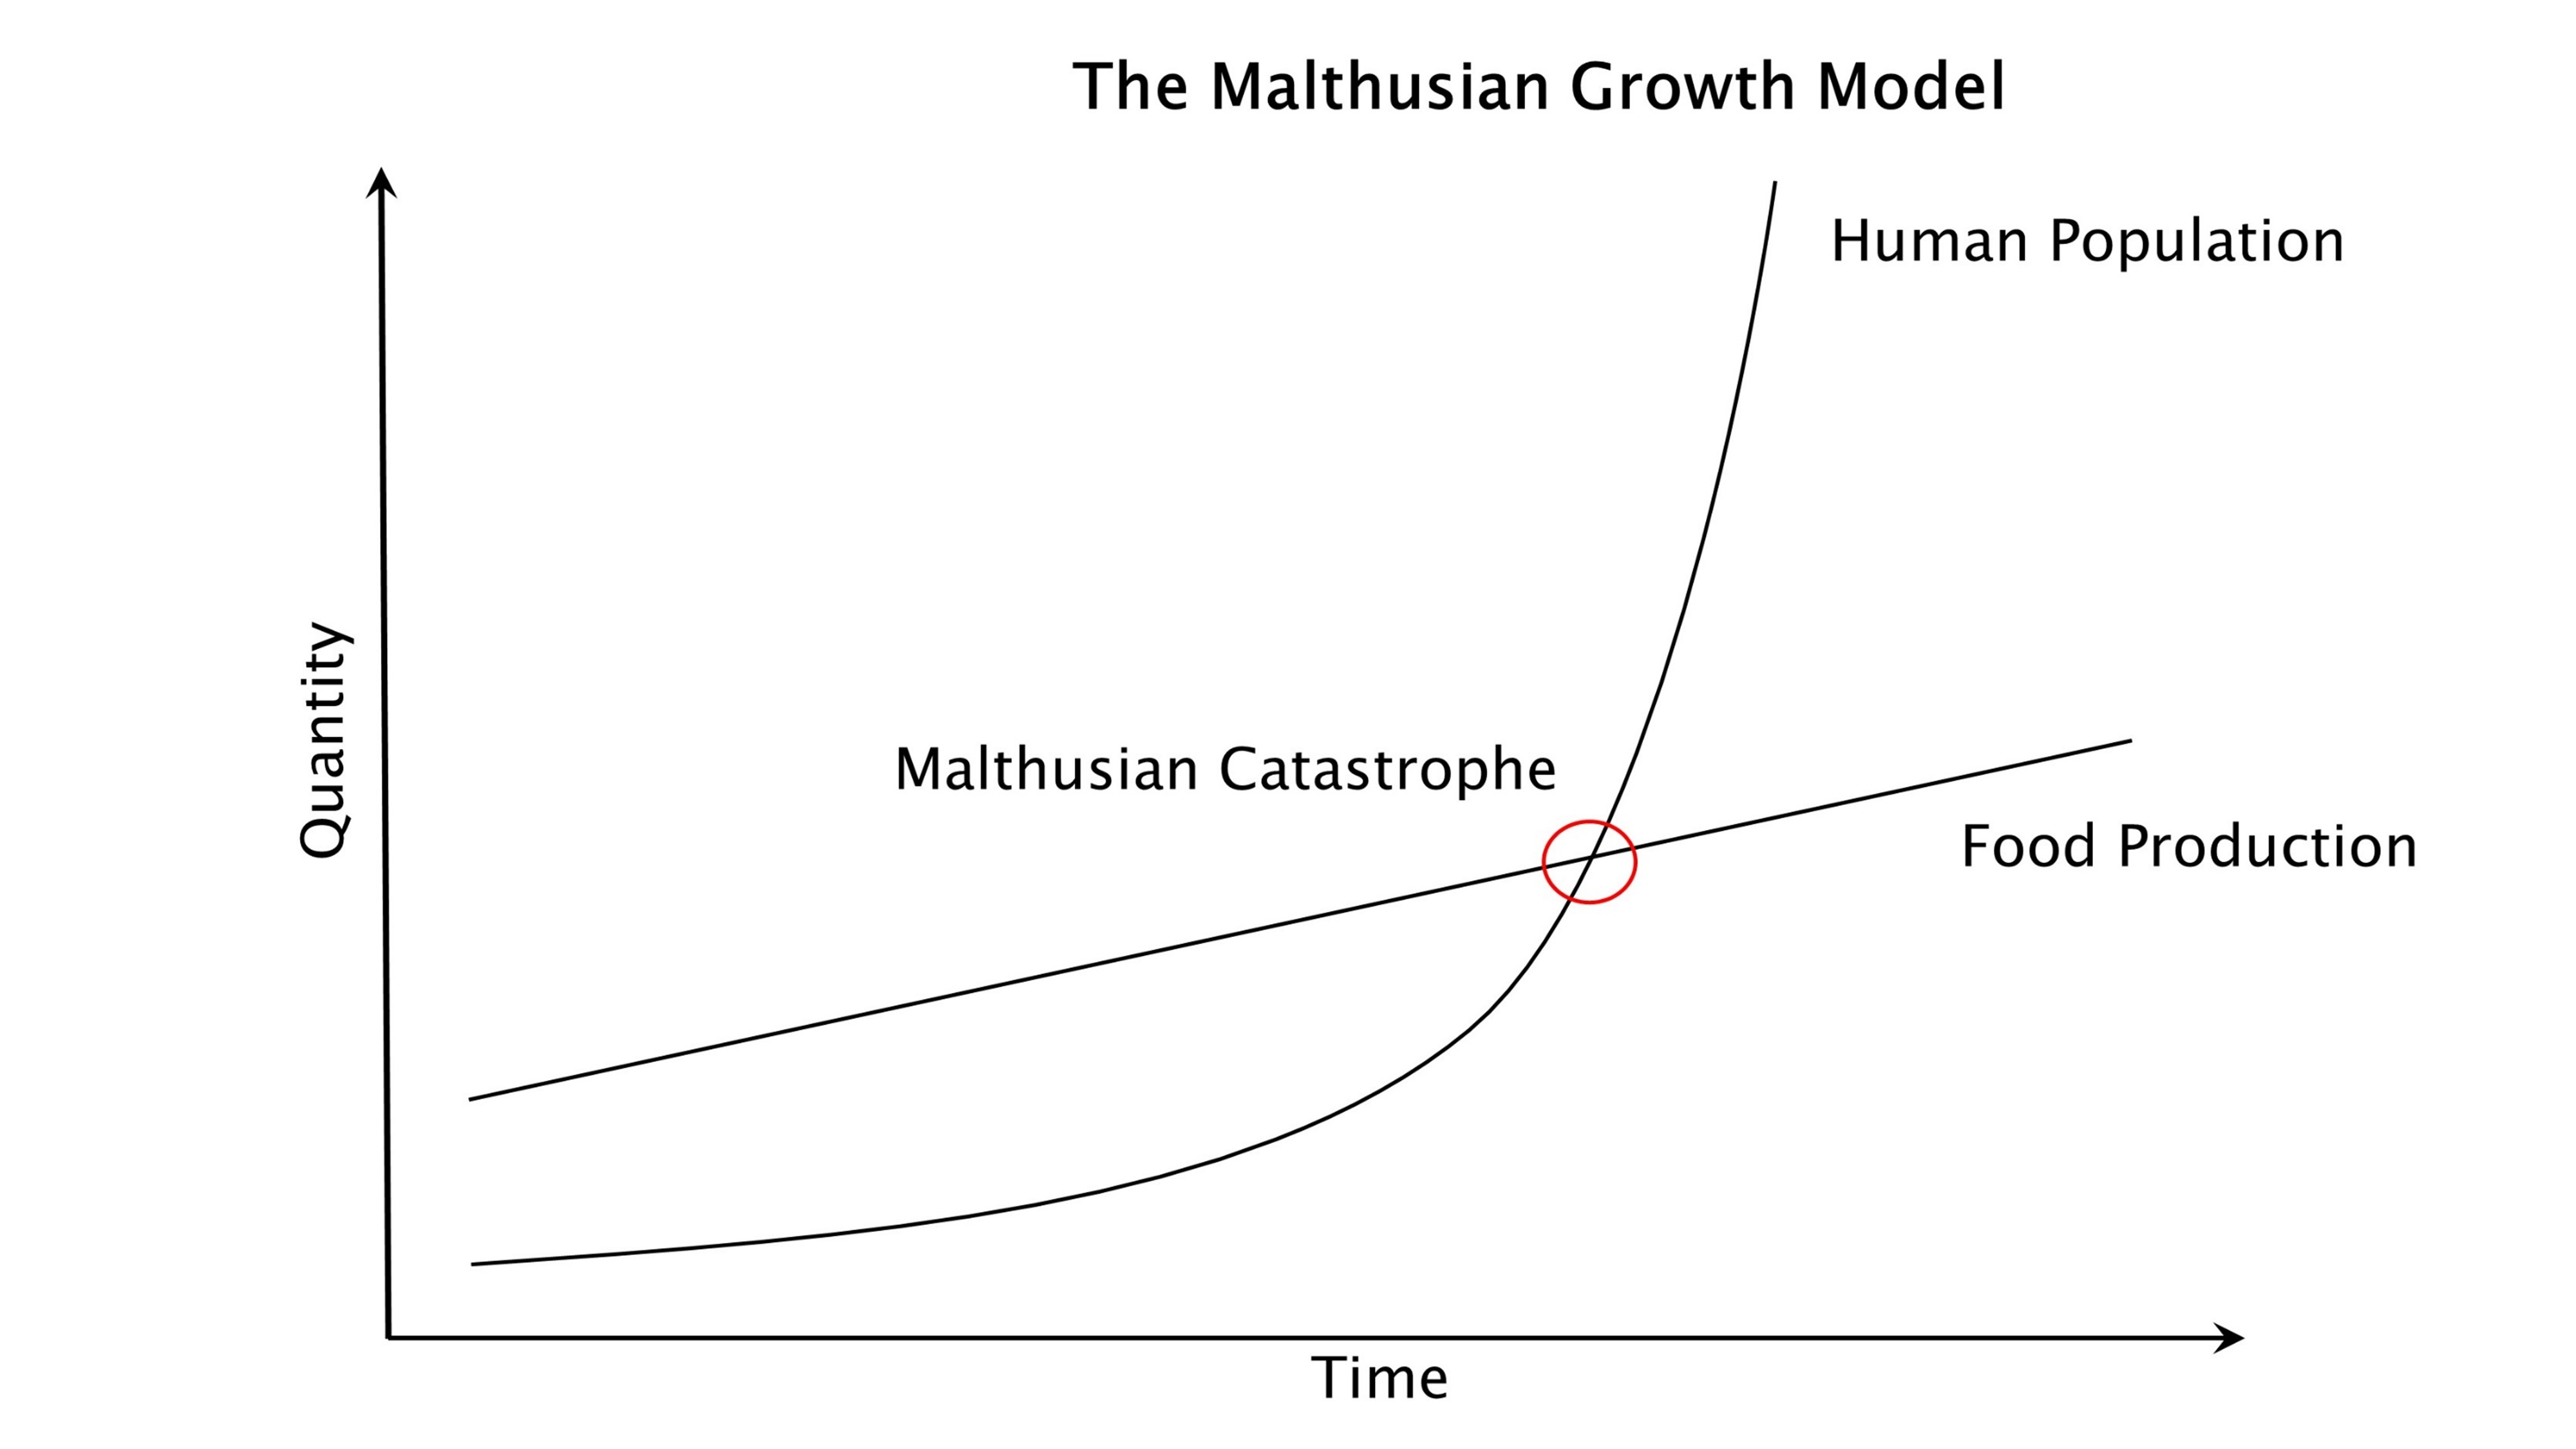
\includegraphics[width=\textwidth]{images/malthus 2.jpg}
    \caption{Supply and demand for food over time.}
    \label{fig:malthus}
\end{figure}

Malthus' argument that food production grows only linearly hinges on decreasing returns to scale in agriculture. If you double the number of farmhands, on a piece of land, you will increase but not double the harvest.

David Ricardo refined the argument. He distinguished between the \emph{internal margin} and the \emph{external margin}. You can increase food production at the internal margin by working crop lands harder. As Malthus noted, this is subject to decreasing returns to scale. At the external margin, you can take virgin lands into crop production. Malthus ignored this. Ricardo did not. Ricardo argued, however, that the external margin would not get around the Malthusian Catastrophe because our ancestors cultivated the best lands first. Expansion on the external margin is thus subject to decreasing quality.

John Stuart Mills further refined the Malthusian argument, nothing that the Catastrophe can be postponed by input substitution. Fertilizers make up for a shortage of soil nutrients, irrigation for a shortfall of rain. However, like Malthus and Ricardo and indeed all Classical Economists, Mills was convinced that economic growth must come to a halt because of resource constraints. 

\subsection{Romanticism}
The Classical economists were sons of the \emph{Enlightenment}. A central part of the Enlightenment was that arguments should be based on observations rather than authority and that decisions should be rational. Economics at the time was typically called \emph{political economy}, a reference to rational, scientifically informed government.

\emph{Romanticism} was a countermovement to the Enlightenment. It was concentrated in the arts, mostly literature (Brontë sisters, François-René de Chateaubriand, Johann Wolfgang von Goethe, Friedrich Schilling, Hendry David Thoreau, William Wordsworth) and to a lesser extent painting (e.g., Caspar David Friedrich) and music (e.g., Johann Sebastian Bach). Romanticists shared three traits. They drew on the older school of Sentimentalism, arguing that emotions are a valid basis for decisions. They harked back to a simpler, better past. And they believed that nature was beautiful and to be enjoyed, rather than dangerous and to be subjugated.

Romanticism had three major offshoots: Communism, Nazism/Fascism, and Environmentalism.

Mao Zedong and Pol Pot took the harking for the past to the extreme, forcing city dwellers to move to the countryside and take up farming. The longing for the past extended to the mighty kings of yore, and the fascists' desire for a strong leader. In that mythical past, everyone was blond with blue eyes. The racial purity of \emph{Blut und Boden} is a key part of Nazism.

Environmentalists tend to argue that things used to be better, and often believe in the myth of the noble savage.\footnote{The noble savage was introduced into modern thought by Michel de Montaigne in 1580. Earlier, in 98, Tacitus had described the Germans as noble savages.} There is a famous quote
\begin{quote}
    Only when the last tree has been cut down, the last fish been caught, and the last stream poisoned, will we realize we cannot eat money.
\end{quote}
This is often presented as a Cree Indian proverb, exemplifying the wisdom and environmental stewardship of pre-modern people.\footnote{It is actually a modern quote of an Abenaki activist who left the reservation at age 7. The quote was popularized by Greenpeace.} In fact, whenever \textit{homo sapiens} introduced itself to a new ecosystem, it wreaked great havoc, including mass extinction.

Environmentalism shares its roots with odious ideologies, but few environmentalists would support them.\footnote{Many fascists love nature, Hitler prime amongst them, Communists less so. Guilt by association is a logical fallacy.} That said, environmentalists tend to be to the political left, but the watermelon epithet\textemdash green on the outside, red on the inside\textemdash is an exaggeration. Some environmentalists argue that democracy is not suited for solving the crisis in the environment. Although the term \emph{eco-fascist} is used with abandon in some circles, there are environmentalists who do not tolerate dissent and pursue their green goals through violent means.

In older literature, danger lurked in the deep dark wood. Romanticists were the first to describe nature as something to be enjoyed rather than feared. This is a reflection of the times. Large predators had mostly disappeared from Western Europe, and you were never far from people. Nature had been tamed and could be enjoyed. People even started swimming in the sea. The oldest environmental organizations began as nature conservation,\footnote{The World Wide Fund for Nature was started to protect the hunting grounds of nobility and royalty.} and emphasized that nature made you a morally better person.

Many people care about the environment but not about Romanticism. The \emph{Ecomodernist} movement explicitly embraces the Enlightenment. It takes positions that are often controversial to environmentalists, arguing for instance that nuclear power is a valid strategy to reduce carbon dioxide emissions and that intensive agriculture is better for nature than the organic sort. Environmental economists are probably more comfortable with ecomodernism while ecological economists tend to associate more with environmentalism.

\subsection{Mill on amenity values}
John Stuart Mill \href{https://www.gutenberg.org/files/30107/30107-pdf.pdf}{(1848, Principles of Political Economy)} brought some Romantic elements into economics,\footnote{Romanticists were fond of Malthus' work, but he was not a Romantic. Malthus was a numbers man, striving for a better future rather than pining for misremembered past and, as all Classical economists, rather wary of a strong government.} writing
\begin{quote}
    There is room in world, no doubt, for a great increase in population, supposing the arts of life to go on improving, and capital to increase. [...] The density of population necessary to obtain all of the advantages both of cooperation and of social intercourse [...] has been attained. A population may be too crowded, though all be amply supplied with food and raiment. [...] Nor is there much satisfaction in contemplating the world with nothing left to the spontaneous activity of nature.
\end{quote}
and adding, for good measure,
\begin{quote}
    it is only in backward countries of the world that increased production is still an important object[ive]
\end{quote}
That is, Mill argued against equating well-being with \emph{material} well-being. This foreshadows Kuznets' admonishment that GDP is a measure of economic activity, not welfare. Mills noted the importance of social intercourse (which we would now rather call interaction) and emphasized the amenity value of nature.

\section{Neo-classical economics}
The neo-classical revolution, led by William Stanley Jevons, Carl Menger and Leon Walras, radically changed economics. The now common tools of partial and general equilibrium and marginal analysis go back to this period.

Although Jevons \href{https://www.econlib.org/library/YPDBooks/Jevons/jvnCQ.html}{(1865, The Coal Question)} worried that
\begin{quote}
    I must point out the painful fact that such a rate of growth will before long render our consumption of coal comparable with the total supply. In the increasing depth and difficulty of coal mining we shall meet that vague, but inevitable boundary that will stop our progress.
\end{quote}
a Malthusian position with coal replacing food\textemdash by and large the neo-classical revolutionaries were hardly interested in issues of environment and resources. This is partly because analysis had moved to the margin, and partly a reflection of the time: Technological progress and industrialization were rapid, and land seemed boundless, with the push into the American west, the Siberian east and the African interior. 

Harold Hotelling was one of the few others neo-classical economists to work on resource problems, developing the rule that the price of an exhaustible resource should rise at the rate of interest. Despite Hotelling's prominence, this work was largely ignored until Robert Solow's 1974 paper and the book by Partha Dasgupta and Geoff Heal of the same year.

Although neo-classical economists paid little attention to the environment, they did lay the foundations for the economic analysis of environmental problems and environmental policy. In 1906, Vilfredo Pareto formulated \emph{Pareto superiority}\textemdash situation A is better than situation B if at least one person is better off and no one is worse off\textemdash \emph{Pareto improvement}\textemdash moving from B to A\textemdash and \emph{Pareto optimality}\textemdash a situation is Pareto optimal if there are no Pareto improvements. Abba Lerner leaned on this and Adam Smith's invisible hand to state the \emph{First Fundamental Welfare Theorem}\textemdash the equilibrium in a perfectly competitive market is a Pareto optimum\textemdash and the \emph{Second Fundamental Welfare Theorem}\textemdash any Pareto optimum can be reached in a perfectly competitive market with the appropriate redistribution of initial endowments. Lerner showed this graphically, the first mathematical proof is due to Hotelling.

Although much of neo-classical analysis was centred on perfectly competitive markets, these economists were not blind to the limitations of this assumption. They just did not know what to do about it. Alfred Marshall, whose 1890 textbook \emph{Principles of Economics} dominated university education, worked on open-access resources.

Marshall also noted that markets were imperfect because of externalities\textemdash an externality is an unintended and uncompensated effect of an economic activity on a third party. It was Alfred Pigou who, in 1920, found the first solution to the problem that externalities pose to the efficiency of the market. Pigou \href{https://www.econlib.org/library/NPDBooks/Pigou/pgEW.html?chapter_num=24#book-reader}{1920, Economics of Welfare, II.XI.11} wrote
\begin{quote}
    If the amount of investment in any industry was carried exactly to the point at which the value of the marginal social net product there is equal to the central value of marginal social net products, the national dividend, so far as that industry is concerned, would be maximised. Disregarding the possibility of multiple maximum positions, I propose, for convenience, to call the investment that would then be made in the industry the ideal investment and the output that would be obtained the ideal output.

    Under conditions of simple competition, if in any industry the value of the marginal social net product of investment is greater than the value of the marginal private net product, this implies that the output obtained is less than the ideal output: if the value of the marginal social net product is less than the value of the marginal private net product, this implies that the output obtained is greater than the ideal output.

    It follows that, under conditions of simple competition, for every industry in which the value of the marginal social net product is greater than that of the marginal private net product, there will be certain rates of bounty, the granting of which by the State would modify output in such a way as to make the value of the marginal social net product there more nearly equal to the value of the marginal social net product of resources in general, thus\textemdash provided that the funds for the bounty can be raised by a mere transfer that does not inflict any indirect injury on production\textemdash increasing the size of the national dividend and the sum of economic welfare; and there will be one rate of bounty, the granting of which would have the optimum effect in this respect.

    In like manner, for every industry in which the value of the marginal social net product is less than that of the marginal private net product, there will be certain rates of tax, the imposition of which by the State would increase the size of the national dividend and increase economic welfare; and one rate of tax, which would have the optimum effect in this respect.
    
    These conclusions, taken in conjunction with what has been said in 
    the preceding paragraphs, create a presumption in favour of State bounties to industries in which conditions of decreasing supply price \textit{simpliciter} are operating, and of State taxes upon industries in which conditions of increasing supply price from the standpoint of the community are operating.
\end{quote}
Pigou argues for the State to intervene to internalize externalities, by imposing taxes on negative ones and subsidies (``bounties'') on positive ones.\footnote{Some students complain about the use of mathematics in economics. Compare and contrast Pigou's definition of the Pigou tax to the one you find in any textbook.}

\section{Keynes and the modern synthesis}
For all the methodological advances in economics, the Great Depression caught the discipline empty-handed. The policy, if you can call it that, of laissez faire had failed. Economics was micro, but the problems of the economy were macro. John Maynard Keynes single-handedly created macroeconomics, focusing on the business cycle and countercyclical government policy.

After World War II, the discipline of economics worked on the \emph{Modern Synthesis} of the recent Keynesian macroeconomics with the older neo-classical microeconomics. One product were the growth models of Harrod and Domar, of Solow, and of Ramsey, Cass and Koopmans. At the core of these models lies the Cobb-Douglas production function, which has that economic output depends on three factors, labour, capital and technology. Natural resources are not there. A one-sector growth model can be interpret as a multi-sector dynamic general equilibrium model if markets are perfect.

In other words, from the start of the neo-classical revolution in 1870 to the end of the modern synthesis in 1970, natural resources and the environment were not part of economics.

\section{Environmental economics}
Things changed in 1970s. As before, economics changed not because of internal pressures but because society changed. After World War II, economic growth was rapid. People could afford cars, and ended up in traffic jams. Those cars emitted gases and particles into the atmosphere. Electricity demand grew rapidly with the use of appliances, and coal-fired power plants added to the pollution of the air. New products were invented, new chemicals developed. The waste of the rapid industrialization was dumped. Rachel Carson published \emph{Silent Spring} in 1962, a book that noted that pesticides weaken egg shells, harming bird reproduction; she predicted a future without birdsong. In 1969, the Cuyahoga River was so polluted it caught fire. In 1972, the Club of Rome published its report of the \emph{Limits to Growth}, a Malthusian tract that predicted society's collapse because of resource constraints well before the average reader of these lecture notes were born. (Hint: It did not happen.) In the same year, the crew of Apollo 17 took the first photo with Earth in full view. Although people had known \emph{intellectually} that our planet is a globe, this was the first \emph{sensory} perception that the Earth is round and finite and we're all in this together. The first oil crises struck in 1973.

After all that, no one could plausibly deny that
\begin{itemize}
    \item natural resources are scarce;
    \item environmental externalities are substantial; and
    \item environmental services are valuable.
\end{itemize}
Environmental economics was born out of that realization. Its aim is to bring the tools of economic analysis to bear on environmental problems and environmental policy.

Kenneth E. Boulding \href{https://www.jstor.org/stable/20024163?seq=1#metadata_info_tab_contents}{reportedly} said
\begin{quote}
    anyone who believes exponential growth can go on forever in a finite world is either a madman or an economist.
\end{quote}
Boulding was a prominent economist, author of a well-read textbook and president of the American Economic Association. He set out his Malthusian views in a 1966 book \emph{The Economics of the Coming Spaceship Earth}.

Nicholas Georgescu-Roegen \href{https://books.google.co.uk/books?hl=en&lr=&id=h1JUarFE1bYC&oi=fnd&pg=PA75&dq=Nicholas+Georgescu-Roegen,+The+Entropy+Law+and+the+Economic+Process&ots=81YMWmd5UJ&sig=WGLF6C6wj1NGn5Uu0r8nqiHjIzc#v=onepage&q=Nicholas\%20Georgescu-Roegen\%2C\%20The\%20Entropy\%20Law\%20and\%20the\%20Economic\%20Process&f=false}{(1971, The Entropy Law and the Economic Process)} wrote
\begin{quote}
    economics gives no signs of acknowledging the role of natural resources in the economic process … the product of the economic process is waste, waste is an inevitable result of that process and ceteris paribus increases in greater proportion than the intensity of economic activity
\end{quote}
Georgescu-Roegen argued that economies are bound by nature (like Boulding), and that models of the economy too should reflect the laws of nature.

Environmental economics took a different route, however. The \emph{Limits to Growth} report had drawn fiery criticism of economists like Graciela Chichilnisky and Bill Nordhaus. In 1980, Julian Simon, a business professor, challenged Paul Ehrlich, a prominent member of the Club of Rome, to a wager. Ehrlich predicted that resource scarcity would drive up the prices of copper, chromium, nickel, tin, and tungsten between 1980 and 1990. Simon predicted a price fall. Simon won.

A common interpretation of the Simon-Ehrlich wager is that human ingenuity is the ultimate resource. We are so clever that we can overcome any challenge that nature might throw of us. This has been true until now. Whether it will be true in the future remains to be seen.

Environmental economics has adopted the position that the tool of economic analysis can be used to analyze environmental problems and that these problems can be solved by changing incentives at the margin.

Ecological economics, on the other hand, takes the position that environmental problems require an overhaul of society and the tools of economics are inadequate.

I am an environmental economist.